\chapter{Deep Learning}

\section{Was ist Deep Learning?}

Unter \textbf{Deep Learning} (zu deutsch tiefes Lernen) versteht man ein Teilgebiet des maschinellen Lernens, welches sich mit künstlichen neuronalen Netzen und große Datenmengen befasst. Es eignet sich für eine Vielzahl von Anwendungsfällen wie beispielsweiße für selbstfahrende Autos, in der Medizin als auch im Marketing. \cite{datasolut2}\\

Mit Deep Learning können Probleme gelöst werden, die ohne diese Ansätze nicht lösbar wären. Tiefes Lernen ist allerdings sehr rechenaufwändig, wodurch das Training über Monate hinweg andauern kann, um gute Entscheidungen treffen zu können. Gründe hierfür sind komplexe Architekturen sowie eine Vielzahl an Modell-Parametern. \cite{datasolut2} \\

\begin{figure}[H]
	\centering
	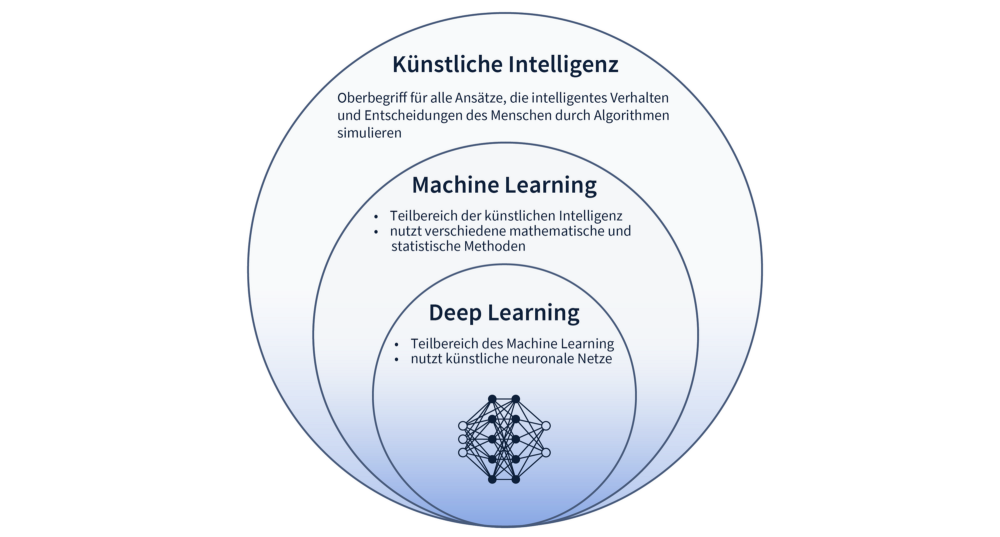
\includegraphics[width=\textwidth]{kapitel3/images/KI_Uebersicht.png}
	\label{fig:ki-übersicht}
	\caption{Übersicht Künstliche Intelligenz}
\end{figure}

Die Grundlage des Deep Learnings stellt die Verwendung von künstlichen neuronalen Netzen dar. Unter künstlichen neuronalen Netzen versteht man Algorithmen, die nach dem biologischen Vorbild des menschlichen Gehirns modelliert sind. Diese werden eingesetzt, um beispielsweise Muster in Bildern zu erkennen oder Bilder zu klassifizieren. \cite{datasolut2}\\

Ein einfaches künstliches neuronales Netz besteht dabei aus einer \textbf{Eingabeschicht} (Input Layer), einer \textbf{Zwischenschicht} (Hidden Layer) und einer \textbf{Ausgabeschicht} (Output Layer). \cite{datasolut2}

\begin{figure}[H]
	\centering
	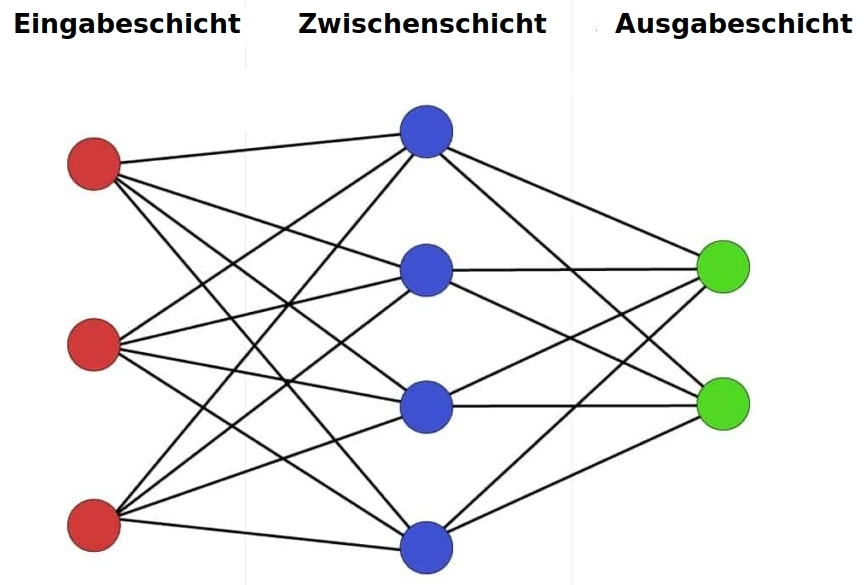
\includegraphics[width=0.65\textwidth]{kapitel3/images/Simples_Neuronales_Netz.jpg}
	\label{fig:simples-neuronales-netz}
	\caption{Darstellung eines beispielhaften künstlichen neuronalen Netzes \\ (vereinfacht)}
\end{figure}

Von tiefem Lernen spricht man dann, wenn die eingesetzen neuronalen Netzte mehr als eine Zwischenschicht haben.  \cite{datasolut2} 

\section{Warum Deep Learning?}

Es gibt Problemstellungen (wie beispielsweise die unstrukturierte Bilderkennung, die sich besonders gut mit künstlichen neuronalen Netzen lösen lassen. Das Erlernen dieser komplexen Muster ist jedoch mit klassischen Machine Leraning Algorithmen nur sehr schwer lösbar. Hier kommen dann tiefe künstliche neuronale Netze zum Einsatz. Je größer die Datenmenge ist, die zum lernen verwendet wird, desto besser funktioniert das tiefe Lernen.

\begin{figure}[H]
	\centering
	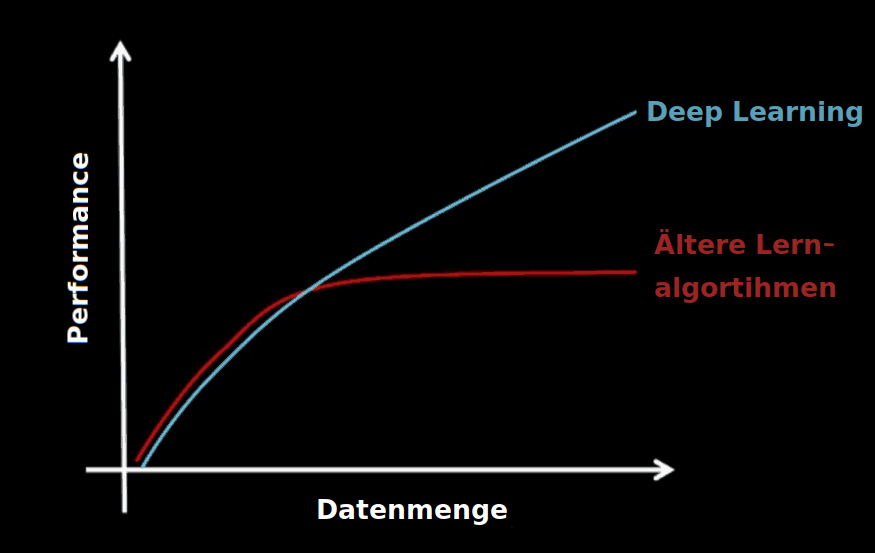
\includegraphics[width=0.65\textwidth]{kapitel3/images/Deep_Learning_Performance.png}
	\label{fig:deep-learning-performance}
	\caption{Darstellung der Performance von Deep Learning Algorithmen im Vergleich zu älteren Lernalgorithmen}
\end{figure}




\section{Problemstellung}

Gegeben sei ein Kamerabild $I_D$, welches von einem Duckiebot $D$ aufgenommen wurde. Das Bild $I_D$ wird einem Posenschätzer $E$ zur Verfügung gestellt, welcher dann den Abstand $d_D$ sowie die Orientierung $\Theta_D$ des Duckiebots zur rechten 
Fahrbahnmarkierung ermitteln soll. Der Posenschätzer ist hierbei ein künstliches neuronales Netz, um die oben genannte Problemstellung lösen zu können. Als Lernverfahren wird überwachtes Lernen eingesetzt.

\section{Datensatzerstellung}

Damit der Posenschätzer seine Aufgabe erfüllen kann, muss zunächst ein Datensatz erstellt werden, damit dieser trainiert werden kann. Der Datensatz besteht dabei aus einem Trainingsdatensatz, einem Validierungsdatensatz sowie aus einem Testdatensatz. \\

Der Trainingsdatensatz ist ein Beispieldatensatz der für das Lernen der Muster und Zusammenhänge in den Daten verwendet wird. Das Modell des neuronalen Netz nutzt also diese Daten um zu lernen. \cite{datasolut} \\

Der Validierungsdatensatz ist ebenso ein Beispieldatensatz, welcher für die Abstimmung der Hyperparameter des Modells des neuronalen Netzes verwendet wird. Dadurch wird das sognenannte \glqq Overfitting\grqq{} (Überanpassung) des Modells auf die Trainingsdaten verhindert. \cite{datasolut} \\

Der Testdatensatz ist ebenfalls ein Beispieldatensatz, jedoch sind die Daten von den Trainingsdaten unabhängig. Die Testdaten werden beim Training des neuronalen Netzes nicht benutzt, sondern dienen zur abschließenden Verifikation des Modells. Dadurch kann die Qualität des Modell erfasst werden, damit man eine Aussage über die Leistungsfähigkeit des neuronalen Netzes treffen kann. \cite{datasolut} \\

Die oben genannten Datensätze wurden mit Hilfe des Duckietownsimulators automatisiert erstellt. Ein Eintrage eines Datensatzes besteht hierbei aus dem Kamerabild $I_D$, welches mit dem dazugehörigen Abstandswert $d_D$ sowie Orientierungswert $\Theta_D$ beschriftet wurde. Der Trainingsdatensatz besteht hierbei aus X Einträgen, der Validierungsdatensatz aus X Einträgen und der Testdatensatz aus X Einträgen. Die Abbildung \ref{fig:data_entry_example} zeigt einige beispielhafte Einträge eines Datensatzes.

\begin{figure}[H]
	\centering
	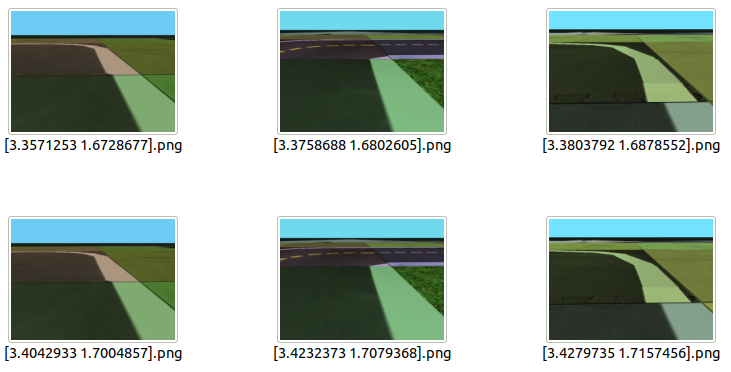
\includegraphics[width=0.8\textwidth]{kapitel3/images/dataset_entries_example.png}
	\caption{Beispielhafte Einträge eines Datensatzes}
	\label{fig:data_entry_example}
\end{figure}


\section{Netzwerkarchitektur}



